\documentclass[12pt,letterpaper]{article}
\usepackage{amsmath,amsthm,amsfonts,amssymb,amscd}
\usepackage{listings}
\usepackage{color}
\usepackage{MnSymbol,wasysym}

\definecolor{dkgreen}{rgb}{0,0.6,0}
\definecolor{gray}{rgb}{0.5,0.5,0.5}
\definecolor{mauve}{rgb}{0.58,0,0.82}

\lstset{%frame=tb,
  language=Bash,
  aboveskip=3mm,
  belowskip=3mm,
  showstringspaces=false,
  columns=flexible,
  basicstyle={\small\ttfamily},
  numbers=none,
  numberstyle=\tiny\color{gray},
  keywordstyle=\color{blue},
  commentstyle=\color{dkgreen},
  stringstyle=\color{mauve},
  breaklines=true,
  breakatwhitespace=true
  tabsize=3
}


\usepackage{hyperref}
\usepackage{graphicx}
\usepackage{enumerate}
\usepackage{fancyhdr}
\usepackage{mathrsfs}
\usepackage[margin=3cm]{geometry}
\setlength{\parindent}{0.0in}
\setlength{\parskip}{0.05in}

% Edit these as appropriate
\newcommand\course{CS595}
\newcommand\semester{FAll 2013}     
\newcommand\hwnum{5}
\newcommand\yourname{Mohamed Aturban}
\newcommand\login{maturban}

\newenvironment{answer}[1]{
  \subsubsection*{Problem #1}
}

\pagestyle{fancyplain}
\headheight 40pt
\lhead{\yourname\ (\login)\\\course\ --- \semester}
\chead{\textbf{\Large Assignment \hwnum}}
\rhead{\today}
\headsep 40pt

\begin{document}

All files mentioned in this document should be uploaded into the {\it github} repository.

\begin{answer}{1}

A Python program, {\it q1\_getFacebookFriendsCount.py}, has been written to extract number of friends that my friends have. The program will search for this information in a file called {\it Mohamed Aturban\_1382319447.graphml} which is created by the Facebook app {\it namegenweb}. Some of my friends' names are in Arabic language, so the function {\it translitArabic} is used to translate Arabic letters to English [1]. The output of this program would be like the following:




\begin{lstlisting}
		Friends-count   Friend-screen-name  
		----------------------------------------
		327             Nabeeh Abdurrahim Hasan
		332             Khaled S. Hatamleh  
		150             Amjad Nusayr        
		93              Fathi M Ben Hamed   
		328             Abdulla Qaddumi     
		140             Riad Ali            
		202             Moad Elgaly         
		...

\end{lstlisting}


The program also produces a vector in R format, so it can be used directly to draw the graph:

\begin{lstlisting}
   (6, 12, 14, 17, 20, 21, 23, 24, 26, 27, 30, 31, 31, 32, 32, 34, 34,
   37, 37, 40, 43, 44, 45, 45, 48, 51, 53, 57, 58, 58, 60, 64, 66, 66,
   67, 68, 68, 69, 75, 78, 78, 79, 80, 84, 85, 85, 86, 89, 90, 92, 93,
   93, 93, 93, 94, 95, 99, 99, 103, 103, 108, 108, 109, 109, 113, 114,
   115, 119, 120, 122, 123, 124, 128, 130, 132, 132, 134, 135, 135, 137,
   139, 139, 140, 141, 142, 142, 143, 147, 150, 158, 159, 160, 160, 161,
   162, 164, 165, 168, 169, 171, 171, 173, 174, 176, 177, 177, 184, 184,
   186, 193, 196, 200, 202, 203, 205, 217, 219, 224, 225, 226, 227, 239,
   239, 249, 251, 253, 269, 270, 276, 283, 295, 310, 319, 327, 328, 332,
   332, 334, 364, 393, 496, 505, 541, 547, 568, 575, 619, 695, 831, 861,
   1037, 3929)
\end{lstlisting}

\begin{figure}[ht!]
\centering
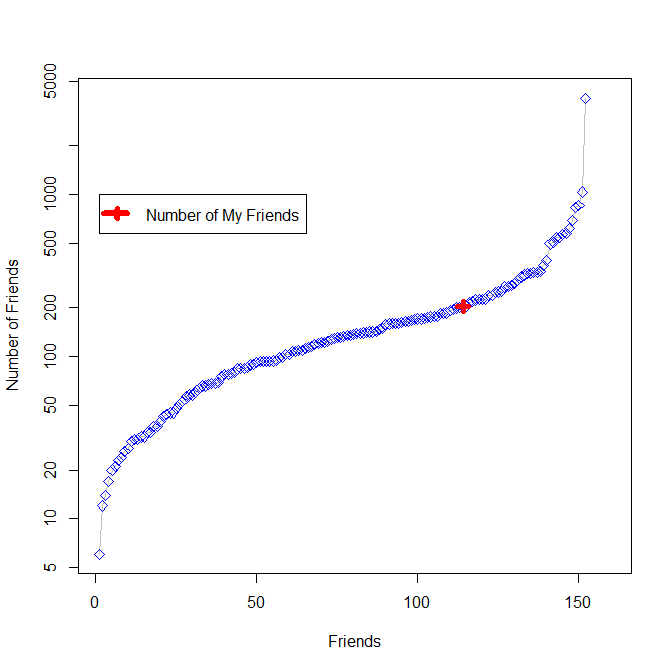
\includegraphics[scale=0.55]{facebook}
\caption{Number of Friends that I and My Friends Have}
\label{overflow}
\end{figure}

I would like to let you know that even though I have 203 friends, only 152 allow me to see their number of friends. This will affect the statistical result. For example, instead of dividing by 203 to get the mean, we divide by 152.


{\bf Some statistics from Figure 1 (calculated in R):}
\begin{itemize}
\item Mean = 197.7434
\item Standard Deviation = 347.0875
\item Median = 133
\item Mohamed Aturban value in ($x-axis, y-axis$) is (114, 203). \smiley{}.
\end{itemize}


Finally, I think the friendship paradox holds for my Facebook account since the mean is equal to 197.7434 which is greater than most of numbers of friends of my friends. In my case, for example, my number of friends is 203 which is close to the mean, and there is 112 numbers out of 152 are less than the mean.

\end{answer}

\begin{answer}{2}

I have done my best to use my Twitter account, but I did not get enough people to follow me; I only have 3 followers; 

Another Python program, {\it q2\_getTwitterFollowersCount.py}, has been written to extract number of followers that Dr. Michael L. Nelson and his followers have. The program will search for this information using Twitter API 1.1.  An application is added to my Twitter account {\it @maturban1}. This app. provides limited access to Twitter data. For example, as user, I was prevented from using this service for an hour because I exceeded 100 requests per hour. Also, to get all followers information I have to deal with the key {\it next\_cursor}. In other words, if a request's response indicates that the value of {\it next\_cursor} is greater than zero, this means more follower data has not been retrieved. In this case, more requests should be issued in order to get this data while if the value of {\it next\_cursor} is zero, no more requests are needed. The output of this program would be like the following:


\begin{lstlisting}
		Followers_count Follower-screen-name Follower-name            
		------------------------------------------------------
		2               amaranaas            anaas                    
		3               maturban1            Mohamed Aturban          
		520             SciTechProf          Christine Borgman        
		10              beatles__beatle      beatles__beatle          
		83              KyleStr              Kyle Strand              
		2               PeterOnymos          Peter Onymos             
		283             MaxJ_K               Max Kemman               
		15              WebSciDL             WS-DL Group, ODU CS      
		84              jakkbl               John Kunze               
		12              samy_tawab           Dr. Samy El-Tawab        
		2074            jschneider           Jodi Schneider           
		102             Milena_Dobreva       Milena Dobreva           
		362             iFromm               Ingo Frommholz   
	   ...

\end{lstlisting}


Same as in question 1, the program also produces a vector in R format, so it can be used directly to draw the graph:

\begin{lstlisting}
  (0, 0, 0, 0, 0, 1, 1, 2, 2, 2, 2, 3, 4, 5, 7, 8, 9, 10, 10, 11, 11,
  11, 12, 12, 12, 12, 12, 15, 15, 19, 20, 20, 21, 21, 22, 25, 26, 26,
  29, 32, 37, 38, 40, 42, 50, 51, 51, 52, 54, 54, 55, 55, 58, 60, 61,
  62, 63, 64, 69, 71, 71, 75, 77, 78, 78, 79, 79, 80, 80, 84, 84, 88,
  90, 90, 91, 94, 96, 99, 102, 103, 104, 109, 109, 110, 119, 121, 121,
  123, 129, 130, 135, 139, 149, 151, 151, 153, 153, 156, 160, 162, 168,
  191, 193, 195, 196, 197, 205, 208, 212, 222, 229, 230, 230, 232, 239,
  241, 246, 253, 259, 265, 268, 268, 269, 282, 283, 293, 294, 318, 321,
  328, 342, 342, 345, 350, 357, 362, 369, 387, 389, 395, 395, 397, 397,
  400, 407, 408, 416, 418, 429, 436, 443, 445, 454, 457, 482, 490, 498,
  499, 517, 520, 545, 556, 562, 565, 569, 578, 586, 593, 622, 625, 640,
  664, 701, 702, 703, 706, 727, 750, 757, 771, 781, 811, 812, 855, 860,
  861, 892, 932, 986, 1032, 1034, 1207, 1252, 1399, 1401, 1440, 1557, 
  1734, 1825, 1929, 1972, 2074, 2455, 2475, 2872, 3502, 9391, 10039, 
  10148)
\end{lstlisting}

\begin{figure}[ht!]
\centering
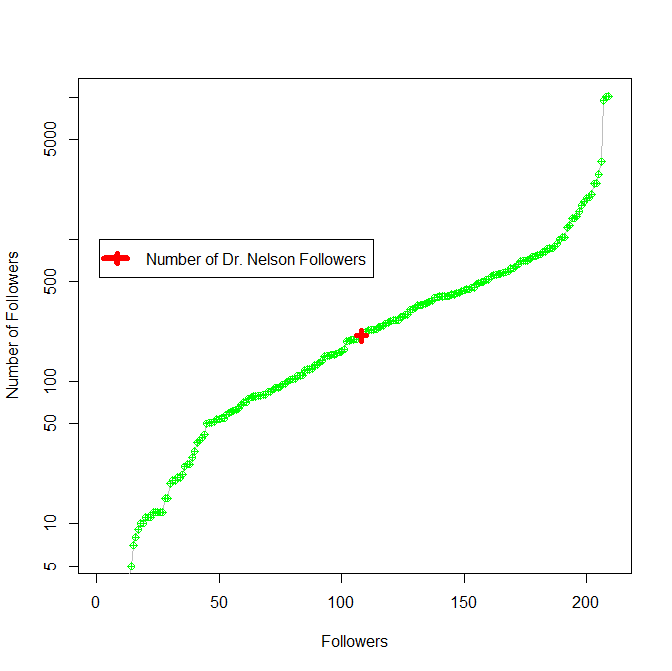
\includegraphics[scale=0.55]{twitter}
\caption{Number of Followers of Dr. Nelson and his followers }
\label{overflow}
\end{figure}


{\bf Some statistics from Figure 2 (calculated in R):}
\begin{itemize}
\item Mean = 513.2536
\item Standard Deviation = 1248.808
\item Median = 196
\item Dr. Nelson value in ($x-axis, y-axis$) is (108, 208). 
\end{itemize}


Finally, I think the friendship paradox holds also for Dr. Nelson Twitter account since the mean is equal to 513.2536 which greater than most of the number of followers of Dr. Nelson's followers. Only about 51 followers have number of followers which is greater than the average while the rest, including Dr. Nelson, have number of followers which is less the average.

\end{answer}

\begin{answer}{3}

Fortunately, {\it linkedIn} provides information about connections (people) through an API (\url{https://www.linkedin.com/secure/developer}. I have written a Python program,
{\it q3\_getLinkedinConnectionsCount}, that requests data from {\it linkedIn} and prints the output as following( I have 24 connections):

\begin{lstlisting}
			Connections     LinkedIn User Name  
			---------------------------------
			202             Fahzy Abdul-Rahman  
			260             Iyad Abu doush      
			256             MAZIN ABUHARAZ      
			154             Saeed Al-Haj        
			500             Anas Al-Tirawi      
			144             Abdussalam Alawini  
			25              Khaled Alharibi     
			15              Espoia Ali          
			70              Adel Altorban       
			99              SAMEH AMMAR         
			13              Ayad Ben-Ismail     
			8               Ibrahim BenMustafa  
			46              Hisham Benotman     
			35              Haythem Gaja        
			52              Abdelrahman Ghuwairi
			365             Bob LaDu,DTM        
			500             Bret Macallan       
			111             Akram Manshalin     
			301             Pilar Montejo       
			305             Elmahdi Omar        
			274             Hisham Turban       
			227             Aimen Younis        
			91              Ayad Zein Eddin     
			7               jlal altrban
\end{lstlisting}



Below are all numbers of connections that my connections have: 
\begin{lstlisting}
	  (7, 8, 13, 15, 24, 25, 35, 46, 52, 70, 91, 99, 111, 144 ,
	  154, 202, 227, 256, 260, 274, 301, 305, 365, 500,500)
\end{lstlisting}

\begin{figure}[ht!]
\centering
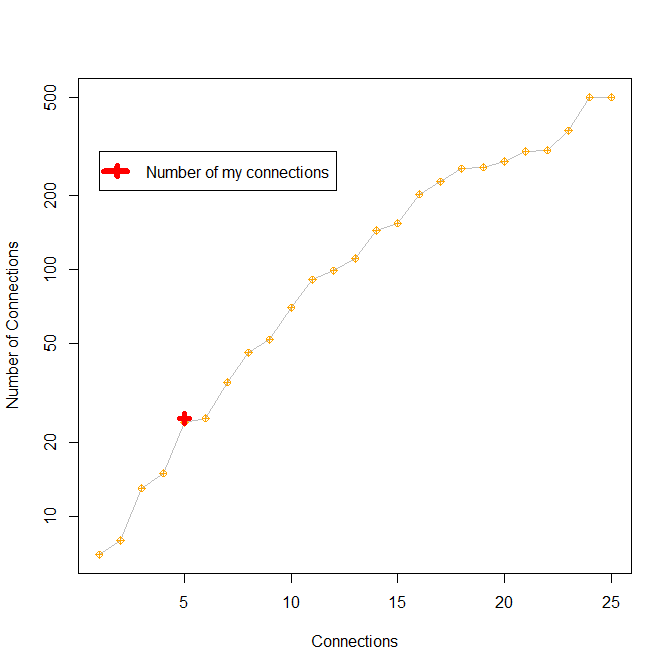
\includegraphics[scale=0.55]{linkin}
\caption{Number of Connections that my Connections have}
\label{overflow}
\end{figure}

{\bf Some statistics from Figure 3 (calculated in R):}
\begin{itemize}
\item Mean = 163.36
\item Standard Deviation = 149.686
\item Median = 111
\item Mohamed Aturban value in ($x-axis, y-axis$) is (5, 24). 
\item I would like indicate here that the API that LinkIn provides returns no more than 500 connection. In other words, if I have someone in my connection has more than 500 connections. LinkIn will give me this person has 500+.

\end{itemize}

I have number of connections which is a way less than the mean, but we can not conclude from the above statistics that the friendship paradox holds for My LinkIn account since must of my connections have connections greater the mean. 

\end{answer}

\begin{answer}{4}

Same instructions explained in question 2 are used to answer this question. As I remember, only one change has been made to {\it q2\_getTwitterFollowersCount.py}. 

\begin{itemize}
\item The old request:
\begin{lstlisting}
...
requests.get(url="https://api.twitter.com/1.1/followers/list.json?
cursor=-1&count=2000&screen_name="+twitterUser+"&skip_status=true&
include_user_entities=false", auth=oauth)
...
\end{lstlisting}
\item After modifying:
\begin{lstlisting}
...
requests.get(url="https://api.twitter.com/1.1/friends/list.json?
cursor=-1&count=2000&screen_name="+twitterUser+"&skip_status=true&
include_user_entities=false", auth=oauth)
...
\end{lstlisting}
\end{itemize}


All new changes are stored in a new file called {\it q4\_getTwitterFollowingCount.py}. The following is the output after running the Python program:
\begin{lstlisting}
	...
	Friends_count   Friends-screen-name  Friends-name             
	-------------------------------------------------
	77              PT_WebArchive        PortugueseWebArchive     
	68              Galsondor            Scott Ainsworth          
	64              weiglemc             Michele Weigle           
	379             neo4j                Neo4j                    
	1203            CommonCrawl          CommonCrawl              
	243             aalsum               Ahmed AlSum              
	107             hanysalaheldeen      Hany SalahEldeen         
	72              justinfbrunelle      Justin F Brunelle        
	366             twarko               Marko A. Rodriguez       
	240             yasmina_anwar        Yasmina Anwar            
	16              WebSciDL             WS-DL Group, ODU CS      
	300             SciTechProf          Christine Borgman        
	...
\end{lstlisting}
\end{answer}


Below are all numbers of following of Dr. Nelson's Following (I am not included \frownie{}): 
\begin{lstlisting}
  (0, 0, 2, 8, 10, 11, 13, 16, 18, 22, 28, 32, 32, 35, 40, 57,
  64, 68, 70, 70, 71, 72, 74, 77, 85, 97, 98, 99, 107, 123, 131,
  133, 139, 161, 176, 178, 192, 198, 202, 224, 240, 241, 243, 245,
  260, 264, 271, 275, 290, 290, 296, 300, 341, 361, 365, 366, 372,
  381, 408, 414, 423, 468, 544, 671, 673, 716, 778, 815, 829, 854,
  860, 985, 1003, 1203, 3351)
\end{lstlisting}

\begin{figure}[ht!]
\centering
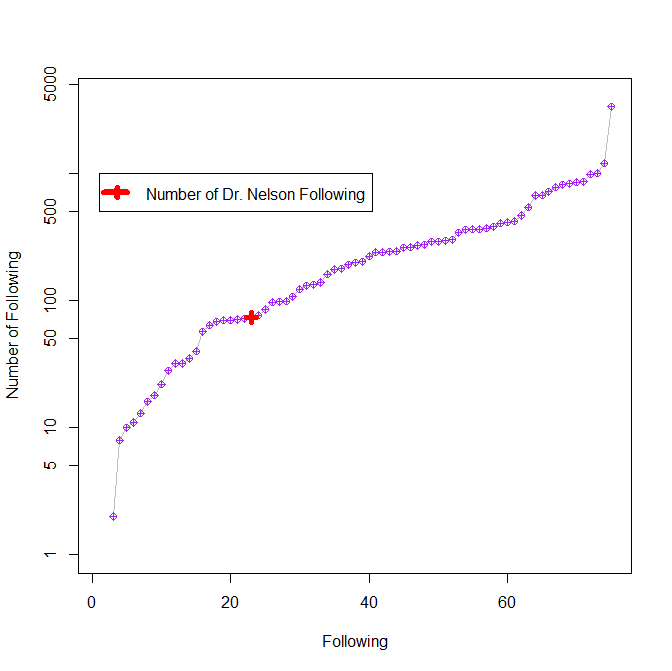
\includegraphics[scale=0.55]{twitter2}
\caption{Number of Following of Dr. Nelson and his following }
\label{overflow}
\end{figure}

{\bf Some statistics from Figure 4 (calculated in R):}
\begin{itemize}
\item Mean =  315.0533
\item Standard Deviation = 452.7505
\item Median = 198
\item Dr. Nelson value in ($x-axis, y-axis$) is (23, 74). 
\end{itemize}

I think here also the friendship paradox holds for Dr. Nelson Twitter account (for following) since the mean is equal to 315.0533 which greater than most of the number of following of Dr. Nelson following including himself. 


References:
[1] http://alraqmiyyat.org/2013/01/python-functions-for-arabic/

\end{document}
